\documentclass[10pt]{beamer}

\begin{document}

\begin{frame}{Recursion activity}

Let's have a list of length \emph{n}:

\begin{center}
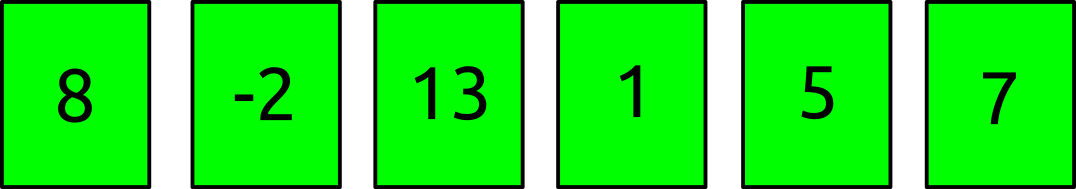
\includegraphics[width=\textwidth]{frames_example.png}
\end{center}

Your task is to \textbf{sort the list using recursion}. Each of you is limited to the following actions:

\begin{enumerate}
\item if anyone \emph{asks me for the help}:
\begin{itemize}
	\item if the list has only one element

	$\rightarrow$ return it to the caller with words: "Here you are"

	\item else

	$\rightarrow$ take the sticky note with \emph{greatest element} from the list and keep it

	$\rightarrow$ ask your neighbour to the help you sort the rest of the list with words: "Please, sort this list for me"
\end{itemize}
\item if anyone returns you a list:
\begin{itemize}
	\item place your sticky note at the end of the list
	\item return your list to the caller with words: "Here you are"
\end{itemize}
\end{enumerate}

\end{frame}

\end{document}